\documentclass[landscape]{standalone}
\usepackage{tikz}
\usetikzlibrary{calc,intersections,through,backgrounds,decorations.pathreplacing,decorations.markings,positioning}
\usepackage{graphicx}
\usepackage{amsmath}
\newcommand*\dif{\mathop{}\!\mathrm{d}}

\def\centerarc[#1](#2)(#3:#4:#5)% [draw options] (center) (initial angle:final angle:radius) 
{ \draw[#1] ($(#2)+({#5*cos(#3)},{#5*sin(#3)})$) arc (#3:#4:#5);}

\begin{document}
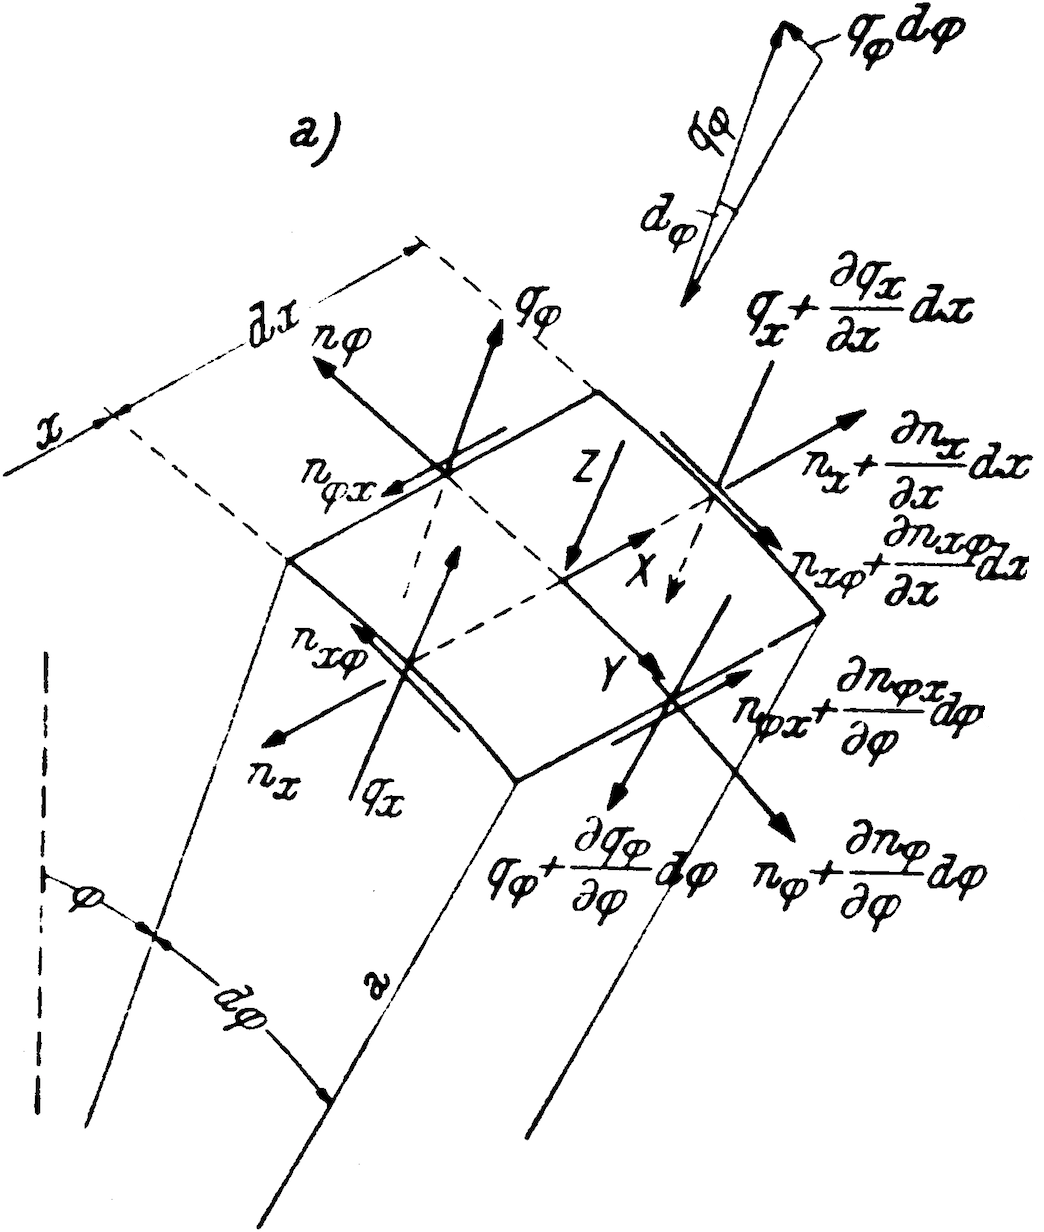
\includegraphics[width=6cm]{sl}\hfill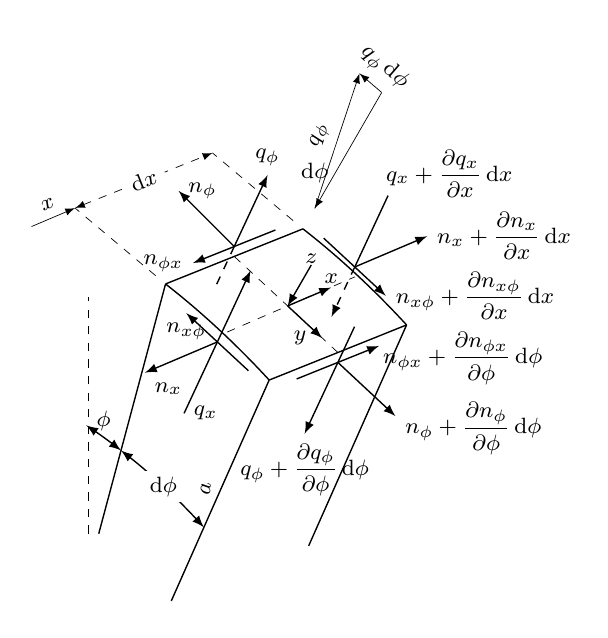
\begin{tikzpicture}[>=latex,line width=0.5pt,thinny/.style={line width=0.25pt},font={\footnotesize}]
% anterior face
\begin{scope}[xslant=0.35,yslant=-0.7]
\draw[] ($(0,0)+({10*cos(95)},{10*sin(95)})$) node (tl1) {} arc (95:85:10) node (tr1) {};
\draw[opacity=0] ($(0,0)+({7*cos(95)},{7*sin(95)})$)   node (bl1) {} arc (95:85:7)  node (br1) {};
\draw[,<->] ($(0,0)+({8*cos(95)},{8*sin(95)})$) arc (95:85:8) node[midway,fill=white,inner sep=2pt] {$\dif\phi$};
\draw[,<->] ($(0,0)+({8*cos(95)},{8*sin(95)})$) arc (95:99:8) node[midway,above,inner sep=2pt] {$\phi$};
\draw[] (bl1.center) -- (tl1.center);
\draw[] (br1.center) -- node[sloped,above] {$a$} (tr1.center);
\end{scope}

% anterior face
\begin{scope}[xslant=0.35,yslant=-0.7,shift={(1.5,1.75)}]
\draw[] ($(0,0)+({10*cos(95)},{10*sin(95)})$) node (tl2) {} arc (95:85:10) node (tr2) {};
\draw[opacity=0] ($(0,0)+({7*cos(95)},{7*sin(95)})$)   node (bl2) {} arc (95:85:7)  node (br2) {};
\draw[] (br2.center) -- (tr2.center);
\end{scope}

\draw (tr1.center) -- (tr2.center);
\draw (tl1.center) -- (tl2.center);
\draw[dashed,thinny] (bl1.west) -- ++(90:3);

\begin{scope}[thinny,dashed]
\draw (tl1) -- ++(140:1.5) node (tll) {};
\draw (tl2) -- ++(140:1.5) node (trr) {};
\end{scope}

\draw[thinny,dashed,<->] (tll.center) -- node[sloped,fill=white] {$\dif x$} (trr.center);
\draw[thinny,<-] (tll.center) -- node[above,sloped] {$x$} ++(203:0.6);


\draw[->] ($(tr1.south)!0.5!(tl1.south)$) -- ++(203:1) node[below right] {$n_{x}$};
\draw[->] ($(tr1.south)!0.2!(tl1.south)$) -- ($(tr1.south)!0.8!(tl1.south)$) node[below] {$n_{x\phi}$};
\draw[->] ($(tr1.south)!0.5!(tl1.south)$) -- ++(65:1);
\draw[] ($(tr1.south)!0.5!(tl1.south)$) -- ++(-115:1) node[right] {$q_{x}$};

\draw[->] ($(tl1.north)!0.5!(tl2.north)$) -- ++(135:1) node[right=0ex and 0ex] {$n_{\phi}$};
\draw[->] ($(tl1.north)!0.8!(tl2.north)$) -- ($(tl1.north)!0.2!(tl2.north)$) node[left=0ex and 0ex] {$n_{\phi x}$};
\draw[->] ($(tl1.north)!0.5!(tl2.north)$) -- ++(65:1) node[above=0ex and 0ex] {$q_{\phi}$};
\draw[dashed]   ($(tl1.north)!0.5!(tl2.north)$) -- ++(-115:0.6);

\draw[->] ($(tr2.north)!0.5!(tl2.north)$) -- ++(23:1) node[right] {$n_{x}+\dfrac{\partial n_x}{\partial x}\dif x$};
\draw[->] ($(tr2.north)!0.8!(tl2.north)$) -- ($(tr2.north)!0.2!(tl2.north)$)  node[right] {$n_{x\phi}+\dfrac{\partial n_{x\phi}}{\partial x}\dif x$};
\draw[] ($(tr2.north)!0.5!(tl2.north)$) -- ++(65:1) node[above right=-1ex and -1ex] {$q_{x}+\dfrac{\partial q_x}{\partial x}\dif x$};
\draw[dashed,->] ($(tr2.north)!0.5!(tl2.north)$) -- ++(-115:0.7);

\draw[->] ($(tr1.south)!0.5!(tr2.south)$) -- ++(-43:1) node[below right=-2ex and 0ex] {$n_{\phi}+\dfrac{\partial n_\phi}{\partial \phi}\dif\phi$};
\draw[<-] ($(tr1.south)!0.8!(tr2.south)$) node[below right=-2ex and -0.5ex] {$n_{\phi x}+\dfrac{\partial n_{\phi x}}{\partial \phi}\dif\phi$} -- ($(tr1.south)!0.2!(tr2.south)$);
\draw[]   ($(tr1.south)!0.5!(tr2.south)$) -- ++(65:0.5);
\draw[->] ($(tr1.south)!0.5!(tr2.south)$) -- ++(-115:1) node[below] {$q_{\phi}+\dfrac{\partial q_\phi}{\partial \phi}\dif\phi$};

%%%%%
\draw[dashed,thinny,name path=l] ($(tr1.center)!0.5!(tr2.center)$) -- ($(tl1.center)!0.5!(tl2.center)$);
\draw[dashed,thinny,name path=r]  ($(tr1.east)!0.5!(tl1.east)$) -- ($(tl2.center)!0.5!(tr2.center)$);
\path[name intersections={of=l and r,by=c}];
\node at (c) {};

\draw[->] (c) -- ++(23:0.6) node[above=-0.5ex and 0ex] {$x$};
\draw[->] (c) -- ++(-43:0.6) node[left=0ex and 0.5ex] {$y$};

\draw[<-] (c.north) -- ++(60:0.6) node[above=-0.7ex and 0ex] {$z$} ;


%%%%%
\draw[opacity=0] (tl2) -- ++(60:2) node (legs1) {};
\draw[opacity=0] (tl2) -- ++(70:2.1) node (legs2) {};

\begin{scope}[->,thinny]
\draw (legs1.center) -- ++(240:1.7) node (lege) {};
\draw (lege.center) -- node[sloped,above] {$q_{\phi}$} (legs2.center);
\draw (legs1.center) -- (legs2.center) node[sloped,midway,above] {$q_\phi \dif\phi$};
\end{scope}
\centerarc[thinny](lege)(60:72:0.7)
\node[above=0.5ex and 0ex of lege,anchor=south] {$\dif\phi$};

\end{tikzpicture}
\end{document}